\documentclass[11pt]{article}

\usepackage[margin=1in]{geometry}
\usepackage[T1]{fontenc}
\usepackage{lmodern}
\usepackage{microtype}
\usepackage{amsmath,amssymb}
\usepackage{booktabs}
\usepackage{graphicx}
\usepackage{xcolor}
\usepackage[numbers,sort&compress]{natbib}
\usepackage{tikz}
\usetikzlibrary{positioning,arrows.meta,fit,calc}
\usepackage[colorlinks=true,linkcolor=blue!60!black,citecolor=blue!60!black,urlcolor=blue!60!black]{hyperref}
\usepackage{cleveref}

\title{\textbf{Hale-Token: Running Data-Center-Scale Mixture-of-Experts LLMs\\on Apple Silicon by Tiering Experts across Unified Memory and SSD}}
\author{B A NaveenKumar\\
\small Independent researcher\\
\small \url{https://github.com/basaanithanaveenkumar/Hale-Token}}
\date{}

\begin{document}
\maketitle

\begin{abstract}
Frontier open-weight language models are sparse mixtures of experts (MoE): Qwen3-235B-A22B
activates 22B of its 235B parameters per token, and DeepSeek-V3 activates 37B of 671B. Most
weights sit idle on any given token, yet standard inference loads all of them, which puts
these models out of reach of laptops. We present \textbf{Hale-Token}, a Rust inference
engine for Apple Silicon (M1--M5) that treats a Mac as a three-tier memory system. The
hottest experts are \emph{pinned} in unified memory, recently used experts live in a
byte-budgeted O(1) \emph{LRU} tier, and every expert is stored on the internal NVMe SSD in a
page-aligned, fixed-stride \emph{pack} that is read with parallel, uncached \texttt{pread}
calls. A closed-form cost model built from the chip's memory bandwidth, core counts, SSD
throughput and RAM sizes the tiers and predicts decode speed before any weights are
downloaded. Routing statistics saved across runs choose which experts to pin. Experts are
quantized to \texttt{q8\_0}/\texttt{q4\_0} with integer dot-product kernels. On a real trained
Mixtral-architecture MoE, logits match Hugging Face \texttt{transformers} to a relative RMS
error of $1.2\times10^{-6}$ (bf16) and 0.42\% (\texttt{q8\_0} experts) with 100\% top-1
agreement. Streaming experts from SSD is bit-identical to fully resident execution. On a
shared Apple M1 CI virtual machine, decoding runs at 26--34 tokens/s with resident experts and
10.3--11.5 tokens/s with only 25\% of experts cached. The same measurements exposed a
thrashing pathology of pure LRU under the cyclic per-layer access pattern of MoE decoding,
which the planner now avoids.
\end{abstract}

\section{Introduction}

Sparse MoE layers~\cite{shazeer2017outrageously,fedus2022switch} decouple model capacity from
per-token compute, and nearly all frontier open models now use them:
Mixtral~\cite{jiang2024mixtral}, DeepSeekMoE and DeepSeek-V3~\cite{dai2024deepseekmoe,deepseekv3},
Qwen3~\cite{qwen3} and Kimi K2~\cite{kimik2}. For a single user decoding one token at a time,
inference is memory-bound: every \emph{active} weight is read once per token. What matters is
therefore where the weights live and how fast each tier can deliver the ones needed next.

On a discrete-GPU PC the critical boundary is the PCIe link between host RAM and VRAM, and
systems such as FlexGen~\cite{sheng2023flexgen}, Mixtral offloading~\cite{eliseev2023offload},
PowerInfer~\cite{song2023powerinfer}, MoE-Infinity~\cite{xue2024moeinfinity} and
FreeToken~\cite{freetoken2026} schedule traffic across it. Apple Silicon removes that boundary:
CPU, GPU and Neural Engine share one pool of unified memory (68\,GB/s on M1 up to 819\,GB/s on
M3 Ultra). The remaining boundary is RAM$\leftrightarrow$SSD, and Apple's internal NVMe drives
read at roughly 3--7\,GB/s. That is 20--100$\times$ slower than memory but fast enough that
streaming only the \emph{missing active experts} each token is practical, as ``LLM in a
flash''~\cite{alizadeh2024flash} showed for dense models.

Hale-Token adapts FreeToken's design to this unified-memory setting. Its contributions:
\begin{itemize}
  \item A \textbf{three-tier expert cache} (pinned, LRU, SSD) with concurrent miss handling
        outside locks, and an \textbf{SSD-optimised expert pack} with O(1) addressing and one
        aligned read per miss (\cref{sec:tiers}).
  \item A \textbf{hardware-aware planner}: a closed-form cost model that sizes the tiers and
        estimates tokens/s for any model on any M-series Mac (\cref{sec:planner}).
  \item A \textbf{placement policy} informed by measurement. A pure LRU smaller than one
        token's working set thrashes under the cyclic layer order of decoding, so small
        budgets pin instead (\cref{sec:results}).
  \item A \textbf{verified implementation}: logits match an independent float64 reference at
        every position and match \texttt{transformers} on a real MoE, and tiering is proven
        bit-identical to resident execution (\cref{sec:verification}).
\end{itemize}

\section{Design}
\label{sec:tiers}

\begin{figure}[t]
\centering
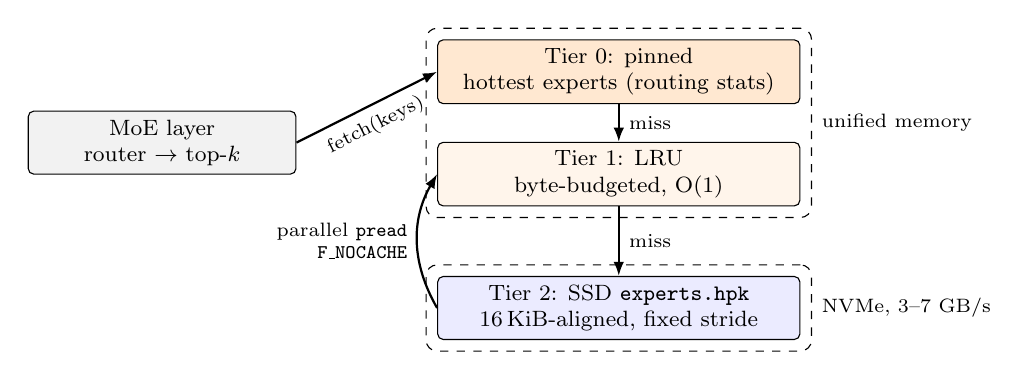
\begin{tikzpicture}[
  box/.style={draw, rounded corners=2pt, align=center, font=\footnotesize, minimum height=8mm, inner sep=3pt},
  arr/.style={-{Latex[length=1.8mm]}, thick}
]
\node[box, fill=gray!10, minimum width=34mm] (moe) at (-0.8,0) {MoE layer\\router $\to$ top-$k$};
\node[box, fill=orange!18, minimum width=46mm] (t0) at (5,0.9) {Tier 0: pinned\\hottest experts (routing stats)};
\node[box, fill=orange!8, minimum width=46mm] (t1) at (5,-0.4) {Tier 1: LRU\\byte-budgeted, O(1)};
\node[box, fill=blue!8, minimum width=46mm] (t2) at (5,-2.1) {Tier 2: SSD \texttt{experts.hpk}\\16\,KiB-aligned, fixed stride};
\node[draw, dashed, rounded corners, fit=(t0)(t1), inner sep=4pt, label={[font=\scriptsize]right:unified memory}] {};
\node[draw, dashed, rounded corners, fit=(t2), inner sep=4pt, label={[font=\scriptsize]right:NVMe, 3--7 GB/s}] {};
\draw[arr] (moe.east) -- node[below, sloped, font=\scriptsize]{fetch(keys)} (t0.west);
\draw[arr] (t0) -- node[right, font=\scriptsize]{miss} (t1);
\draw[arr] (t1) -- node[right, font=\scriptsize]{miss} (t2);
\draw[arr] (t2.west) to[bend left=30] node[left, font=\scriptsize, align=right]{parallel \texttt{pread}\\\texttt{F\_NOCACHE}} (t1.west);
\end{tikzpicture}
\caption{Expert tiers. Misses are read concurrently from the SSD pack and inserted into the LRU.}
\label{fig:tiers}
\end{figure}

\paragraph{Model execution.} Hale-Token implements decoder-only MoE transformers (Qwen3-MoE and
Mixtral) on the CPU. It uses RMSNorm, grouped-query attention with QK-norm and RoPE, an
append-only KV cache, and MoE layers in which a router selects the top-$k$ experts with a
bounded min-heap ($O(n\log k)$) and sums their weighted SwiGLU outputs. Dense weights
(attention, norms, embeddings, routers) keep their checkpoint precision and are loaded
zero-copy through \texttt{mmap} of safetensors files. Activations and accumulations are
\texttt{f32}. For quantized weights the activation vector is quantized to 8 bits once per
mat-vec and dotted with integer arithmetic, following llama.cpp's block
formats~\cite{llamacpp}. The kernels compile to NEON \texttt{sdot} on every M-series chip.
Rows and heads are reduced in a fixed order, so results are deterministic regardless of
thread count or cache placement.

\paragraph{Tiers.} The model sees only an \texttt{ExpertProvider::fetch(keys)} interface
(\cref{fig:tiers}). The cache (i)~records the routing decision, (ii)~looks each key up in the
pinned tier and then the LRU, (iii)~reads \emph{all} misses concurrently from the SSD, keeping
the NVMe queue full, and (iv)~inserts the loaded experts into the LRU, evicting by bytes. Two
short mutex sections bracket the lookup and the insert. All I/O happens outside the locks.
The LRU is a hash map plus a doubly linked list stored in a slab, giving O(1) get, insert
and evict with no allocation in steady state.

\paragraph{Expert pack.} Loading experts through \texttt{mmap} of the original checkpoint works
but is wasteful. The OS evicts by page recency, bf16 experts are $3.5\times$ larger than
\texttt{q4\_0}, the three matrices of one expert are scattered across the file, and pages would
be held both in the page cache and in the expert cache. \texttt{hale convert} therefore writes
\texttt{experts.hpk}: a magic string, a JSON header (dtype, sizes, MoE layer list, record size,
stride) and fixed-size records $[\text{gate}\,|\,\text{up}\,|\,\text{down}]$ aligned to
Apple Silicon's 16\,KiB page. A record's offset is
$\text{base} + (\ell\cdot E + e)\cdot\text{stride}$, so no index is needed, and a miss costs
exactly one aligned \texttt{pread}. \texttt{F\_NOCACHE} prevents double caching in the unified
buffer cache. The converter writes records in parallel with positional writes.

\section{Planner}
\label{sec:planner}

The planner is a pure function from (model shape, hardware, dtypes) to a placement and a
speed estimate. With $B_d$ dense bytes, $B_e$ bytes per expert, $A_e$ active expert bytes
per token, and RAM share $0.75$:
\begin{align}
  R_e &= 0.75\,\mathrm{RAM} - B_d - 2\,\mathrm{GB}, &
  h &\ge \min\!\big(R_e/B_e,\ N_e\big)/N_e \quad\text{(uniform-routing floor)},\\
  t_{\text{mem}} &= \frac{B_d + h\,A_e}{0.6\,\mathrm{BW}_{\text{mem}}}, &
  t_{\text{cpu}} &= \frac{2\,P_{\text{active}}}{\mathrm{FLOPS}}, \qquad
  t_{\text{ssd}} = \frac{(1-h)\,A_e}{\mathrm{BW}_{\text{ssd}}},\\
  t_{\text{token}} &= \max(t_{\text{mem}}, t_{\text{cpu}}) + t_{\text{ssd}} .
\end{align}
SSD time is additive because a layer cannot start before its experts arrive. CPU throughput
is modelled as 24\,GFLOP/s per performance core and 6 per efficiency core. The default SSD
bandwidth is a conservative 5\,GB/s, and the efficiency factor of 0.6 reflects achievable
CPU bandwidth. A built-in table of M1--M5 chips (bandwidth, core counts, RAM options) lets
\texttt{hale plan} answer ``what can my Mac run?'' before a download. \Cref{tab:plan}
reproduces its output.

\paragraph{Placement.} If every expert fits, all are pinned. If the budget is smaller than two
tokens' working set ($2\times$ MoE layers $\times k$ experts), every slot is pinned and no LRU
is used (see \cref{sec:results}). Otherwise the budget is split evenly between pinned and LRU.
Pinned experts are the hottest according to \texttt{hale-routing.json}, selected with
quickselect. Without history, they are spread evenly across layers.

\begin{table}[t]
\centering
\caption{Planner estimates of decode tokens/s (\texttt{q4\_0} experts, bf16 dense weights, SSD at
5\,GB/s), reproduced with \texttt{hale plan --compare}. RAM: all experts resident. SSD: streamed.
--: dense weights do not fit. SSD figures are floors that assume uniform routing.}
\label{tab:plan}
\small
\setlength{\tabcolsep}{4pt}
\resizebox{\linewidth}{!}{%
\begin{tabular}{lrrrrrr}
\toprule
Model (total / active) & M1 16G & M2 Pro 32G & M4 Pro 64G & M4 Max 128G & M2 Ultra 192G & M3 Ultra 512G \\
\midrule
Qwen3-30B-A3B (30.5B / 3.3B) & 4.9 S & 29.4 R & 39.5 R & 46.7 R & 64.6 R & 93.4 R \\
Mixtral-8x7B (46.7B / 12.9B) & 0.9 S & 2.2 S & 10.3 R & 12.1 R & 16.8 R & 24.2 R \\
Mixtral-8x22B (141B / 39B) & -- & 0.3 S & 0.4 S & 4.0 R & 5.5 R & 8.0 R \\
Qwen3-235B-A22B (235B / 22B) & -- & 0.6 S & 0.7 S & 1.3 S & 8.1 S & 14.1 R \\
DeepSeek-V3$^\ast$ (671B / 37.5B) & -- & -- & 0.4 S & 0.5 S & 0.6 S & 4.1 S \\
Kimi-K2$^\ast$ (1.03T / 32.6B) & -- & -- & 0.4 S & 0.4 S & 0.5 S & 1.0 S \\
\bottomrule
\end{tabular}}\\[2pt]
{\footnotesize $^\ast$Plannable but not yet executable (multi-head latent attention).}
\end{table}

\section{Verification}
\label{sec:verification}

Correctness is checked at five levels. \textbf{Unit} tests cover kernels, quantization, the
LRU, top-$k$, the planner and the pack format. \textbf{Litmus} tests compare logits at
\emph{every} position against an independent NumPy float64 implementation (full-sequence
attention versus our incremental KV cache) and require identical greedy tokens, on tiny
Mixtral and Qwen3-MoE fixtures. \textbf{Tiering} tests stream experts from the SSD pack
through a one-expert cache and require logits bit-identical to fully resident execution.
Quantized packs must stay within error bounds. \textbf{CLI} tests exercise \texttt{convert},
\texttt{run}, \texttt{plan}, \texttt{bench} and \texttt{logits} end to end, and a
\textbf{cross-check} script compares \texttt{hale logits} with Hugging Face
\texttt{transformers}. The whole suite runs in CI on arm64 macOS runners. It also passes on
Linux x86\_64: 49 unit tests plus all integration tests.

\section{Results}
\label{sec:results}

All measurements come from the repository's CI on a GitHub \texttt{macos-14} runner (a shared
3-vCPU Apple M1 virtual machine). They use the real trained MoE
\texttt{Isotonic/TinyMixtral-4x248M-MoE} (Mixtral architecture, 12 layers $\times$ 4 experts,
top-2) with the prompt ``The capital of France is''.

\begin{table}[t]
\centering
\caption{Measured on a GitHub \texttt{macos-14} runner (Apple M1 VM) with TinyMixtral-4x248M-MoE.}
\label{tab:measured}
\resizebox{\linewidth}{!}{%
\begin{tabular}{ll}
\toprule
Check & Result \\
\midrule
\texttt{hale logits} vs \texttt{transformers} (bf16) & rel.\ RMS error $1.2\times10^{-6}$, top-1 agreement 100\% \\
\texttt{hale logits} vs \texttt{transformers} (\texttt{q8\_0} experts) & rel.\ RMS error 0.42\%, top-1 agreement 100\% \\
Greedy output & ``Paris. France is the capital of France. \ldots'' \\
Decode, experts resident (\texttt{q8\_0}) & 26--34 tokens/s \\
Decode, SSD-streamed, cache = 25\% of experts & 10.3--11.5 tokens/s, hit rate 18\%, SSD 4.2--5.3 GB/s \\
\bottomrule
\end{tabular}}
\end{table}

\Cref{tab:measured} summarises the results. Numerically, the engine matches the reference
implementation to within bf16 rounding, and \texttt{q8\_0} experts change logits by under half a
percent without changing any top-1 prediction. With three quarters of the experts on SSD,
decoding still runs at roughly a third of the resident speed.

\paragraph{LRU thrashing.} The first placement policy used a pure LRU for small budgets.
With a cache of 25\% of the experts it achieved a \textbf{0\% hit rate} and read 11.9\,GB from
the SSD per 32 tokens. Every token visits the MoE layers in the same order, so expert accesses
are cyclic, and an LRU smaller than the cycle evicts each expert just before it is needed
again, the classic worst case for LRU. Pinning a fixed set of the same size instead yields an
18\% hit rate (close to the 25\% uniform-routing expectation) and 9.7\,GB of reads. The planner
now pins whenever the budget is below two tokens' working set.

\paragraph{Caveat on absolute speed.} On the CI VMs \texttt{hale bench memory} measures only
7--10\,GB/s against 68\,GB/s on a physical M1, and kernel benchmarks vary by up to
$3\times$ between runs. The measured speeds are therefore lower bounds. Physical-hardware
measurements of Qwen3-30B-A3B and Qwen3-235B-A22B are future work.

\section{Limitations and Future Work}

Execution is CPU-only. A Metal backend would use the GPU's share of unified-memory bandwidth.
Prefill processes tokens one at a time. Multi-head latent attention and shared experts
(DeepSeek-V3, Kimi K2) can be planned but not yet run. Pre-quantized formats (GPTQ, AWQ, FP8,
GGUF) are not read, so conversion starts from bf16 releases. The planner's SSD estimates
assume uniform routing and are therefore pessimistic for real, skewed routers.

\section{Conclusion}

Unified memory changes the offloading problem from PCIe scheduling to RAM/SSD tiering.
Hale-Token shows that with a page-aligned expert pack, concurrent uncached reads, a
bandwidth-aware planner and a placement policy that respects the cyclic access pattern of
MoE decoding, frontier-scale MoE models become runnable on a Mac, with correctness verified
at every position.

\paragraph{Acknowledgements.} The design follows FreeToken~\cite{freetoken2026}. Quantized block
layouts follow llama.cpp~\cite{llamacpp}.

\bibliographystyle{plainnat}
\bibliography{references}

\end{document}
